% !TeX spellcheck = de_DE
\section{Evaluation}
Nachdem die Parallelisierung der Evaluationsphase durchgeführt und die Testumgebung spezifiziert ist, wird in diesem Kapitel die Performance des Verfahrens gemessen. Die hierbei erhaltenen Ergebnisse werden mit denen der sequenziellen Implementierung verglichen. Im letzten Schritt wird eine Bewertung bezüglich der Effizienz und des \emph{SpeedUps} abgegeben.

\subsection{Mountain Car}
\label{subsec:mountain_car_optimzation}
Das parallelisierte Verfahren wird zuerst in der \emph{Mountain Car} Umgebung getestet, die aus Kapitel \ref{subsec:analysis_mountain_car} bekannt ist. Mit dem Ziel, einen einfachen Vergleich zwischen der sequenziellen und parallelisierten Implementierung zu ermöglichen, wird die zuvor verwendete Konfiguration des Verfahrens vollständig übernommen. Selbiges gilt für den \emph{Seed}. Bei korrekter Implementierung des parallelisierten Verfahrens werden dieselben Zwischenergebnisse nach jeder Generation generiert und das finale Ergebnis wird mit dem des sequenziellen Verfahrens übereinstimmen. Somit kann keine Implementierung einen zeitlichen Vorteil erlagen, der durch bessere Agenten oder kürzere Evaluationszeiten entsteht. Beide Implementierungen werden dieselben Berechnungen und Evaluationen durchführen.
\begin{figure}[!h]
	\centering
	\begin{minipage}[]{0.49\textwidth}
		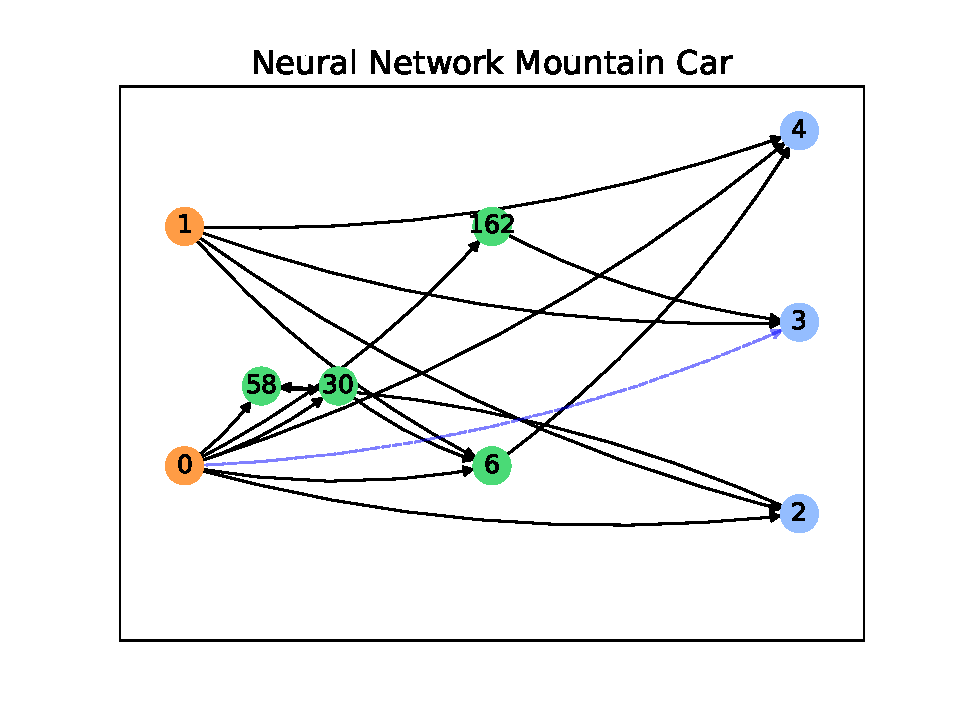
\includegraphics[width=1.0\textwidth]{./img/mountain_car_single/mountain_car_neural_network.pdf} 
	\end{minipage}
	\hfill
	\begin{minipage}[]{0.49\textwidth}
		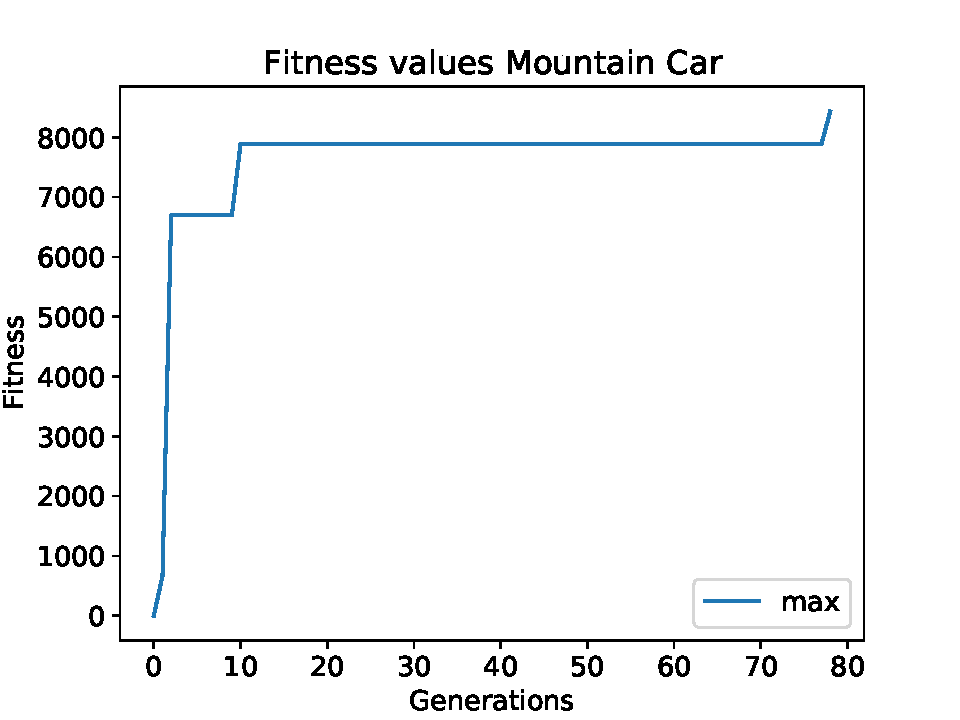
\includegraphics[width=1.0\textwidth]{./img/mountain_car_single/1413_fitness_1core_1pi.pdf} 
	\end{minipage}
	\caption{Links die Lösung für das Mountain Car Problem, rechts die dazugehörigen Fitnesswerte pro Generation mit 10 Prozessen}
	\label{fig:mountain_car_10core_neural_network_and_fitness}
\end{figure}
\begin{figure}[!h]
	\centering
	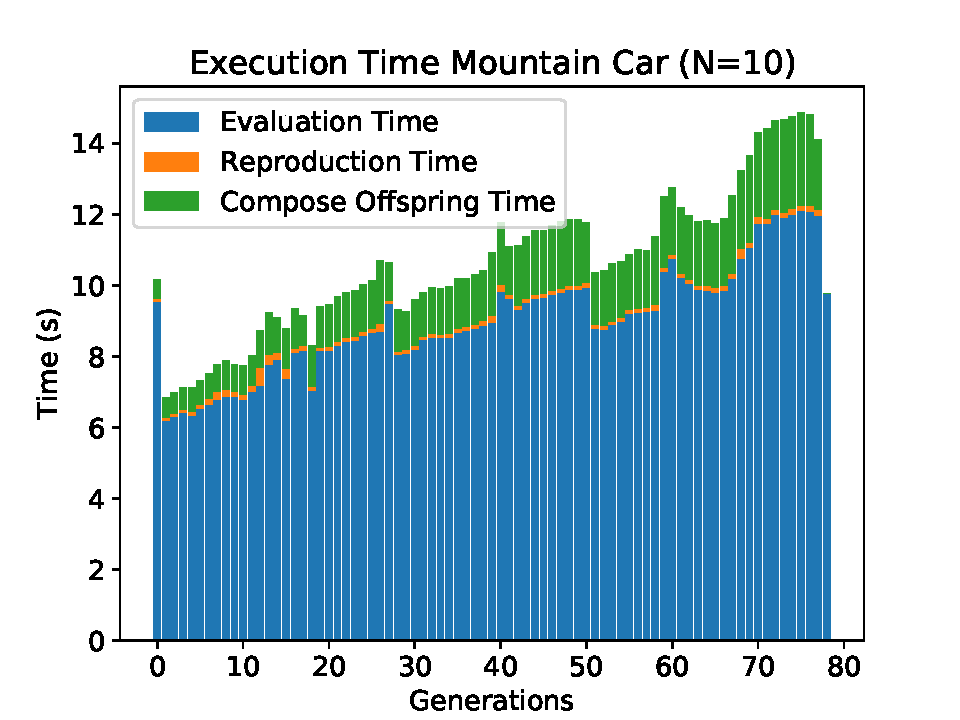
\includegraphics[width=0.7\textwidth]{./img/mountain_car_analysis/1413_time_10cores_10pis.pdf} 
	\caption{Ausführungszeit des \emph{Mountain Car} Problems auf 10 \emph{Raspberry Pis} mit 10 Prozessen}
	\label{fig:mountain_car_time_10cores_10pi}
\end{figure}
\\\\
Im ersten Durchlauf wird der parallelisierte Algorithmus mit zehn Prozessen auf zehn Raspberry Pis ausgeführt. Das Verfahren ist so konfiguriert, dass auf jedem Raspberry Pi ein Prozess gestartet wird. Abbildung \ref{fig:mountain_car_10core_neural_network_and_fitness} zeigt das hierbei entstandene \ac{KNN} und den maximal erreichten Fitnesswert. Beide Darstellungen sind identisch mit denen des sequenziellen Verfahrens. Da auch die restlichen Zwischenergebnisse übereinstimmen, wie beispielsweise die Anzahl an verschiedenen Spezies pro Generation, ist die Anforderung bezüglich des \emph{Seeds} erfüllt. Sowohl die parallelisierte als auch die sequenzielle Implementierung führen dieselben Rechenschritte aus, wodurch ein direkter Vergleich der Laufzeiten möglich ist. Die Ausführungszeit für die vorgestellte Konfiguration ist in Abbildung  \ref{fig:mountain_car_time_10cores_10pi} dargestellt. Wie beim sequenziellen Verfahren wird diese in die Phasen \emph{Evaluation Time}, \emph{Reproduction Time} und \emph{Compose Offspring Time} unterteilt. Grundsätzlich ist festzustellen, dass die insgesamt benötigte Laufzeit stark verringert ist. Mit zehn Prozessen in der vorgestellten Konfiguration sinkt die durchschnittliche Rechenzeit auf ungefähr $10.5$ Sekunden pro Generation. Die sequenzielle Implementierung hat im Vergleich dazu etwa $80$ Sekunden pro Generation benötigt. Für die gesamte Ausführungszeit des Verfahrens bedeutet dies, dass das parallelisierte Verfahren bereits nach $14$ Minuten beendet ist. Im Vergleich zur Laufzeit der sequenziellen Implementierung mit $105$ Minuten, ist das parallelisierte Verfahren $91$ Minuten schneller.
\\\\
Eine Besonderheit des Graphen zeigt sich in der ersten Generation. In dieser ist die Ausführungszeit der \emph{Evaluation Time} vergleichsweise hoch. Der Grund hierfür ist, dass das Starten und Initialisieren der beteiligten Prozesse Zeit benötigt, welche die Evaluation der Agenten verzögert. Da dies im Rahmen der \emph{Evaluation Time} erfasst wird, erhöht sich die gemessene Ausführungszeit in der ersten Generation. Für die nachfolgenden Generationen trifft dies nicht mehr zu, da die Initialisierung nur einmalig zu Beginn erfolgt. Eine weitere Besonderheit betrifft die Form des Graphen. Wie bei der sequenziellen Implementierung gibt es auch in der parallelisierten Implementierung Generationen, in denen die Ausführungszeit stark sinkt oder ansteigt. Mögliche Gründe hierfür sind in Kapitel \ref{subsec:analysis_mountain_car} erörtert. Bei einem direkten Vergleich der Ausführungszeiten ist festzustellen, dass diese Änderungen meistens in denselben Generationen auftreten. Diese Eigenschaft ist wichtig, da ein Vergleich der Laufzeiten nur möglich ist, wenn die Messergebnisse, abgesehen von kleinen Abweichungen, konsistent sind. Diese Eigenschaft kann zusätzlich mit der \emph{Reproduction Time} und \emph{Compose Offspring Time} verifiziert werden. Diese Phasen sind nicht parallelisiert und daher sollte die Ausführungszeit identisch sein. Insgesamt sind die gemessenen Laufzeiten in diesen Phasen etwas höher als bei der sequenziellen Implementierung. Über alle $78$ Generationen entsteht eine Differenz von ungefähr $5$ Sekunden beziehungsweise $4\%$. Diese Unterschiede können beispielsweise durch Hintergrundprozesse im Betriebssystem entstehen, auf welche kein Einfluss genommen werden kann. Da die Abweichungen insgesamt gering sind, kann dennoch ein Vergleich der Laufzeiten vorgenommen werden. Die letzte zu nennende Eigenschaft bezüglich der Abbildung \ref{fig:mountain_car_time_10cores_10pi} ist der prozentuale Anteil der \emph{Reproduction Time} und \emph{Compose Offspring Time}. Bei der sequenziellen Implementierung haben diese beiden Phasen nur etwa $2\%$ der Ausführungszeit in Anspruch genommen. Im aktuellen Testdurchlauf sind dies $15\%$, da durch die Parallelisierung der Anteil der \emph{Evaluation Time} sinkt. Aufgrund \emph{Amdahl's Law} ist anzunehmen, dass durch das Hinzufügen von weiteren Prozessen der prozentuale Anteil der \emph{Reproduction Time} und \emph{Compose Offspring Time} weiter ansteigt.
\begin{figure}[!h]
	\centering
	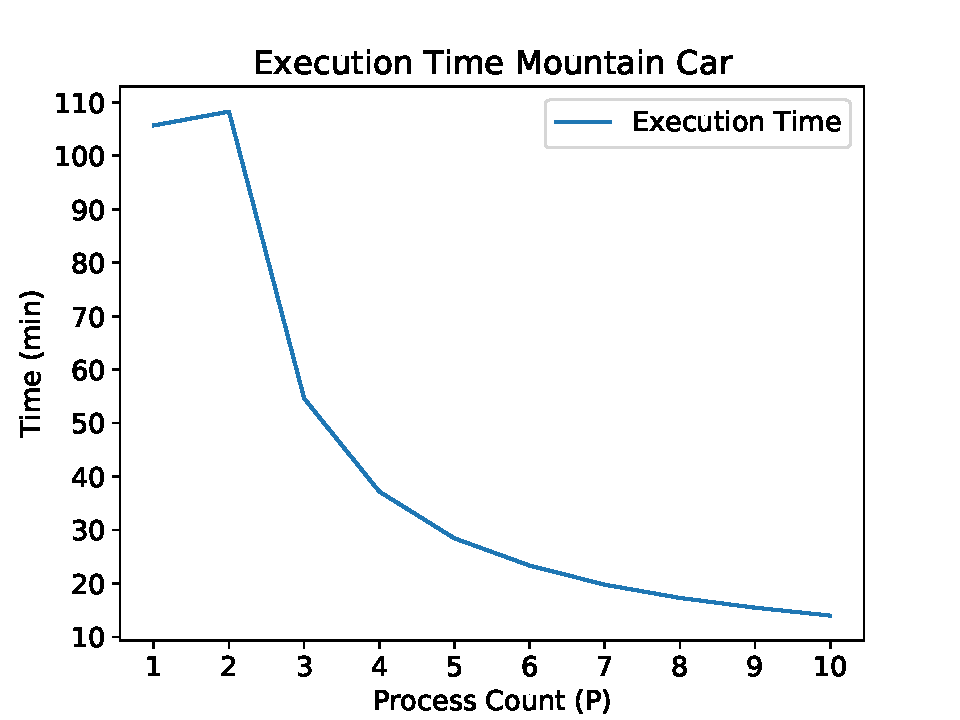
\includegraphics[width=0.7\textwidth]{./img/mountain_car_analysis/time_mountain_car_1_10.pdf} 
	\caption{Ausführungszeit des parallelisierten Verfahrens in der \emph{Mountain Car} Umgebung in Abhängigkeit der Prozessanzahl}
	\label{fig:execution_time_mountain_car_1_10}
\end{figure}
\\\\
Für eine vollständige Bewertung des parallelisierten Verfahrens werden die in Kapitel \ref{subsec:basics_performance} vorgestellten Metriken \emph{SpeedUp} und Effizienz benötigt. Für eine bessere Einordnung der Ergebnisse werden diese nicht nur für die oben vorgestellte Konfiguration mit zehn Prozessen, sondern auch für Testdurchläufe mit zwei bis neun Prozessen berechnet. Diese werden im Folgenden mit derselben Konfiguration durchgeführt. Die hierbei entstehenden \ac{KNN} und Fitnesswerte sind identisch mit den vorherigen und sind daher nicht abgebildet. Die benötigte Ausführungszeit für das gesamte Verfahren in Abhängigkeit zur Anzahl an Prozessen ist in Abbildung \ref{fig:execution_time_mountain_car_1_10} dargestellt. Eine Besonderheit hierbei ist, dass die benötigte Ausführungszeit mit zwei Prozessen länger ist als mit einem Prozess. Der Grund hierfür liegt in der gewählten \emph{Master-Slave} Architektur des parallelisierten Verfahrens. Mit einem Prozess wird das sequenzielle und andernfalls das parallelisierte Verfahren ausgeführt. Werden genau zwei Prozesse verwendet, gibt es einen \emph{Master} und einen \emph{Slave}. In diesem Fall ist die Ausführung langsamer als beim sequenziellen Verfahren, da der \emph{Master} im Rahmen der Parallelisierung nur die Kommunikation koordiniert, selbst aber keine Aufgabenpakete abarbeitet. Der \emph{Slave} führt alleine die Evaluation der Agenten durch. Dafür benötigt er dieselbe Zeit wie das sequenzielle Verfahren. Hinzu kommt der benötigte Kommunikationsaufwand, für das Verteilen der Agenten und Sammeln von Fitnesswerten. Aufgrund der hierfür aufgewendeten Zeit ist das parallelisierte Verfahren mit zwei Prozessen langsamer als das sequenzielle Verfahren. Mit drei oder mehr beteiligten Prozessen sinkt die Ausführungszeit kontinuierlich. 
\begin{figure}[!h]
	\centering
	\begin{minipage}[]{0.49\textwidth}
		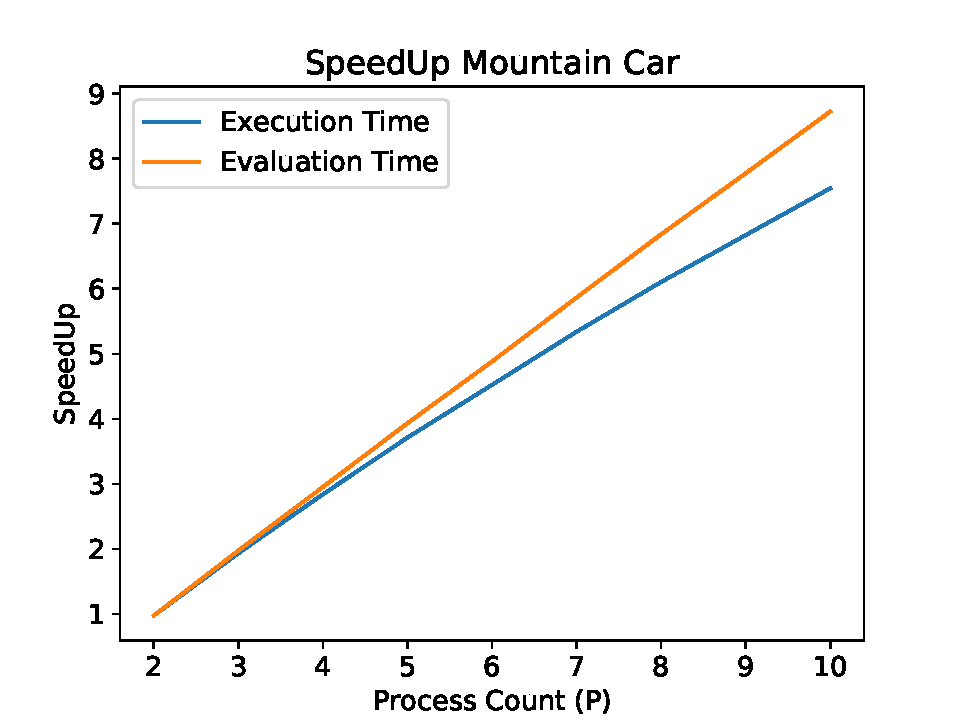
\includegraphics[width=1.0\textwidth]{./img/mountain_car_analysis/mountain_car_speedup_2_10.pdf} 
	\end{minipage}
	\hfill
	\begin{minipage}[]{0.49\textwidth}
		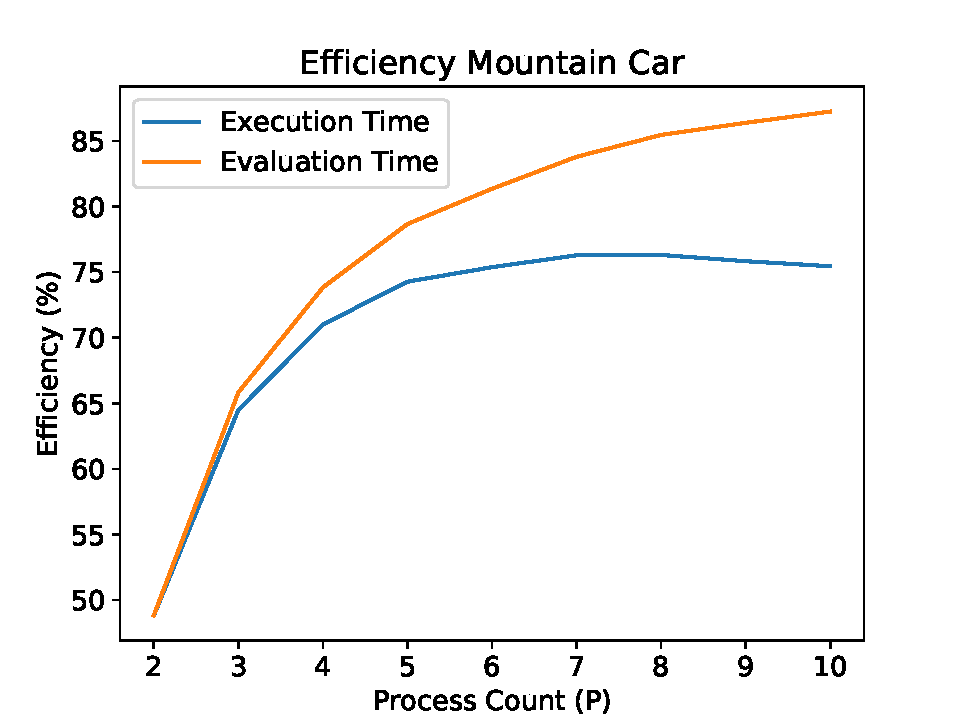
\includegraphics[width=1.0\textwidth]{./img/mountain_car_analysis/efficecny mountain_car_2_10.pdf} 
	\end{minipage}
	\caption{Links der \emph{SpeedUp}, rechts die dazugehörigen Effizienzwerte für die \emph{Mountain Car} Umgebung in Abhängigkeit der Prozessanzahl}
	\label{fig:mountain_car_2_10_efficiency_speedup}
\end{figure}
\\\\
Anhand der Ausführungszeiten wird der \emph{SpeedUp} und die Effizienz des parallelisierten Verfahrens gemessen, welche eine Bewertung der Implementierung ermöglichen. Abbildung \ref{fig:mountain_car_2_10_efficiency_speedup} zeigt links die erreichten \emph{SpeedUps} und rechts die dazugehörigen Effizienzwerte in Abhängigkeit zur Anzahl an verwendeten Prozessen. In beiden Graphen sind jeweils die Metriken für die Evaluationsphase und das gesamte Verfahren dargestellt. Beim Testdurchlauf mit zehn Prozessen ist das parallelisierte Verfahren ungefähr um den Faktor $7.6$ schneller als das sequenzielle Verfahren. Dieses Ergebnis ist grundsätzlich höher als bei den vorherigen Testdurchläufen mit weniger Prozessen, entspricht aber nicht der Vorhersage von \emph{Amdahl's Law}. Laut diesem liegt der maximal erreichbare \emph{SpeedUp} mit zehn Prozessen in einem zu $98\%$ parallelisierbaren Programm bei ungefähr $8.5$. Durch die gewählte \emph{Master-Slave} Kommunikationsarchitektur ist zwischen dem erwarteten und tatsächlich erhaltenen Wert eine Differenz von $0.9$. Wie bereits beschrieben, unterstützt der \emph{Master} die \emph{Slaves} nicht bei der Evaluation, wird aber dennoch bei den Berechnungen berücksichtigt. Wird nur die Anzahl der \emph{Slave} Prozesse bei der Berechnung von \emph{Amdahl's Law} verwendet, ergibt sich ein maximaler \emph{SpeedUp} von $7.8$. Die restliche Differenz von $0.2$ entsteht durch den Kommunikationsaufwand. 
\begin{figure}[!h]
	\centering
	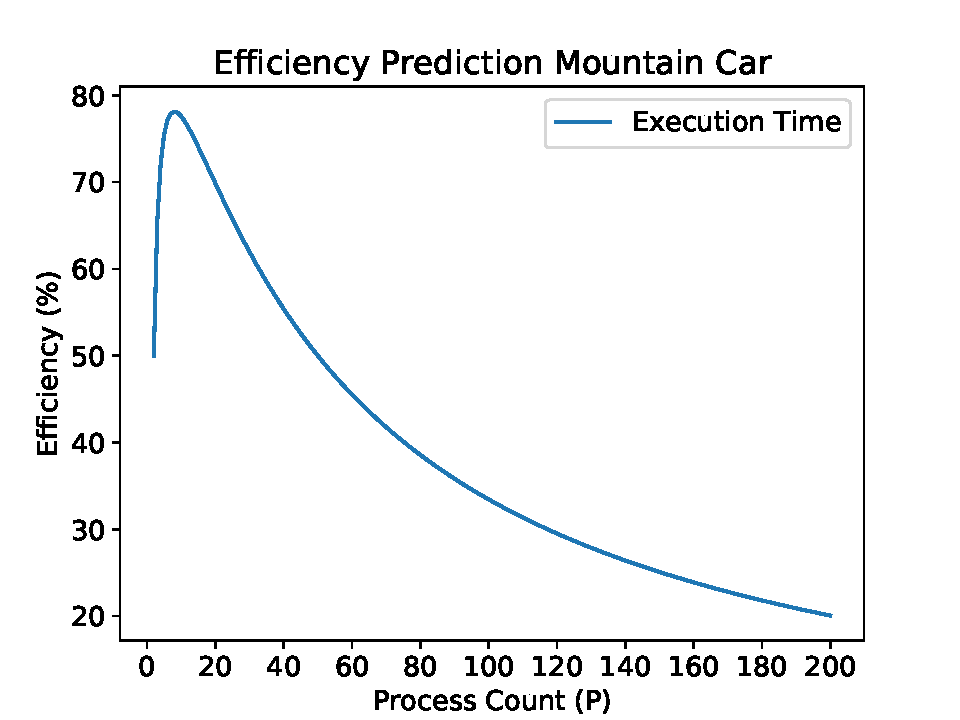
\includegraphics[width=0.7\textwidth]{./img/mountain_car_analysis/mountain_car_efficiency_prediction.pdf} 
	\caption{Erwartete Effizienz in der \emph{Mountain Car} Umgebung in Abhängigkeit der Anzahl an Prozessen}
	\label{fig:mountain_car_efficiency_predidction}
\end{figure}
\\\\
Die in Abbildung \ref{fig:mountain_car_2_10_efficiency_speedup} rechts dargestellten Effizienzwerte beurteilen den \emph{SpeedUp} anhand der Prozessanzahl. Initial erzielt das parallelisierte Verfahren mit zwei Prozessen aufgrund der \emph{Master-Slave} Architektur eine geringe Effizienz. Mit je einem \emph{Master} und \emph{Slave} wird entsprechend der Abbildung \ref{fig:execution_time_mountain_car_1_10} eine etwas höhere Ausführungszeit im Vergleich zur sequenziellen Implementierung benötigt. Daher liegt der \emph{SpeedUp} bei ungefähr $0.98$. Entsprechend der Formel aus Kapitel \ref{subsec:basics_performance} ergibt die Berechnung der Effizienz einen Wert von $49\%$. Beim Hinzufügen weiterer Prozesse sinkt der Einfluss des \emph{Masters} auf das Ergebnis und die Effizienz steigt. Mit sechs bis zehn Prozessen wird ein Wert von über $75\%$ erreicht. Aufgrund des Graphen und \emph{Amdahl's Law} ist davon auszugehen, dass der Wert nicht weiter steigen, sondern durch Hinzufügen weiterer Prozesse letztendlich sinken wird. Abbildung \ref{fig:mountain_car_efficiency_predidction} zeigt die erwarteten Effizienzwerte für die \emph{Mountain Car} Umgebung mit einer \emph{Master-Slave} Architektur, wobei die Werte mit \emph{Amdahl's Law} berechnet worden sind. Auch in diesem Fall steigt die Effizienz anfangs stark an. Der höchste Wert von ungefähr $78\%$ wird mit acht Prozessen erreicht. Dies entspricht etwa dem tatsächlich erhaltenen Ergebnis. Hierbei wird die höchste Effizienz von $76\%$ ebenfalls mit acht Prozessen erreicht. Der Grund für das starke Absinken der Effizienz im weiteren Verlauf ist darin begründet, dass der \emph{SpeedUp} durch den sequenziellen Anteil von \emph{Amdahl's Law} immer gegen einen bestimmten Wert konvergiert. Die niedrigen Effizienzwerte entstehen, da der \emph{SpeedUp} nicht proportional zur Anzahl der Prozesse ansteigt.
\\\\
Es ist möglich, den \emph{SpeedUp} und die Effizienz nur für die parallelisierte \emph{Evaluation Time} zu berechnen, sodass der sequenzielle Teil des Verfahrens keinen Einfluss auf das Ergebnis hat. Die Ergebnisse hiervon sowie die des gesamten Verfahrens sind in Abbildung \ref{fig:mountain_car_2_10_efficiency_speedup} dargestellt. Der \emph{SpeedUp} der \emph{Evaluation Time} ist nahezu linear. Mit neun \emph{Slaves} bzw. zehn Prozessen wird ein \emph{SpeedUp} von $8.7$ erreicht. Diese guten Ergebnisse spiegeln sich in der Effizienz wieder. Diese ist anfänglich durch die \emph{Master-Slave} Architektur bei $49\%$, steigt aber stetig an. Mit zehn Prozessen liegt sie bei $87\%$. Prinzipiell kann der Wert weiter ansteigen, da der Einfluss des \emph{Masters} auf das Ergebnis mit zunehmender Prozessanzahl sinkt. Dennoch ist aufgrund der entstehenden Kommunikationszeit keine Effizienz von $100\%$ möglich. Bleibt bei der Effizienzberechnung der \emph{Master} Prozess unberücksichtigt, werden Ergebnisse zwischen $97\%$ und fast $99\%$ erreicht. Dies entspricht nahezu dem idealen Wert.

\subsection{Pendulum}
In diesem Kapitel wird die \emph{Pendulum} Umgebung mit dem parallelisierten Verfahren evaluiert und bewertet. Zusätzlich werden die Ergebnisse mit denen des vorherigen Kapitels verglichen. Hierzu wird das Optimierungsproblem zunächst in verschiedenen Testdurchläufen mit zwei bis zehn Prozessen optimiert und die \emph{Evaluation Time}, \emph{Reproduction Time} und \emph{Compose Offspring Time} für jeden von diesen erfasst. Die Konfiguration und der \emph{Seed} werden vom sequenziellen Verfahren übernommen, sodass alle Testdurchläufe dieselben Lösung produzieren und ein Vergleich der Implementierungen möglich ist. Wie bei der \emph{Mountain Car} Umgebung, wird von jedem Raspberry Pi maximal ein Prozess ausgeführt. 
\begin{figure}[!htb]
	\centering
	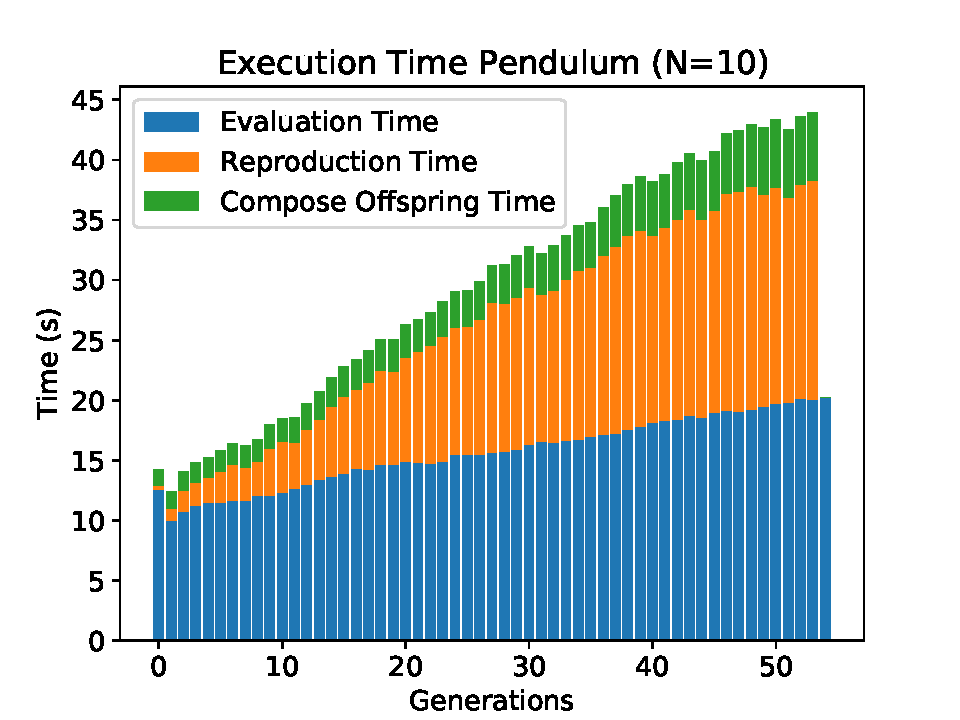
\includegraphics[width=0.7\textwidth]{./img/pendulum_analysis/pendulum_time_1_10core_10pi.pdf} 
	\caption{Ausführungszeit des \emph{Pendulum} Problems auf 10 \emph{Raspberry Pis} mit 10 Prozessen}
	\label{fig:pendulum_time_10cores_10pi}
\end{figure}
\\\\
Die Ergebnisse zeigen, dass die Fitnesswerte und die finalen \ac{KNN} identisch zum sequenziellen Verfahren sind, daher werden sie hier nicht abgebildet. Der Schwerpunkt der Analyse liegt auf den Ausführungszeiten. Diese sind für den zuletzt durchgeführten Test mit zehn Prozessen in Abbildung \ref{fig:pendulum_execution_time_1_10} dargestellt. Wie bei der \emph{Mountain Car} Umgebung ist die \emph{Evaluation Time} der ersten Generation im Vergleich zur zweiten höher. Der Grund hierfür ist die Initialisierung der einzelnen Prozesse.  Die gesamte Ausführungszeit beträgt in diesem Test $27$ Minuten. Im Vergleich zur sequenziellen Implementierung, welche $138$ Minuten benötigt hat, ist dies eine Zeitersparnis von $111$ Minuten. Zuletzt ist bezüglich dieses Graphen hervorzuheben, dass die \emph{Evaluation Time} im Verlauf der Generationen nur leicht ansteigt und insgesamt $53\%$ der Ausführungszeit ausmacht. Der Anteil der anderen beiden Phasen ist anfänglich gering, steigt aber stark an und benötigten in den letzten Generationen zusammen mehr Zeit als die eigentliche Evaluation. Wie bereits beim sequenziellen Verfahren beschrieben, ist der Grund für die vergleichsweise hohe \emph{Reproduction Time} die hohe Anzahl an verschiedenen Spezies. 
\begin{figure}[!htb]
	\centering
	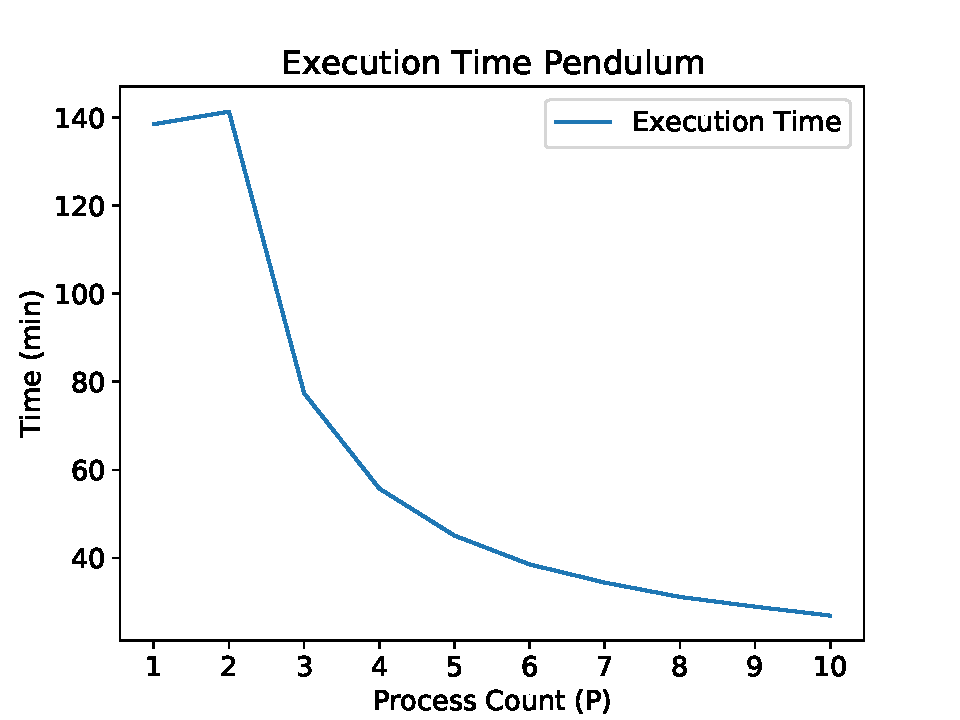
\includegraphics[width=0.7\textwidth]{./img/pendulum_analysis/pendulum_execution_1_1_10.pdf} 
	\caption{Ausführungszeit des parallelisierten Verfahrens in der \emph{Pendulum} Umgebung in Abhängigkeit der Prozessanzahl}
	\label{fig:pendulum_execution_time_1_10}
\end{figure}
\\\\
Als nächsten wird der Verlauf der gesamten Ausführungszeit in Abhängikeit der Anzahl an Prozessen betrachtet. Diese sind in Abbildung \ref{fig:pendulum_execution_time_1_10} dargestellt. Prinzipiell ähnelt der Graph dem der \emph{Mountain Car} Evaluation. Mit zwei Prozessen steigt die Ausführungszeit im Vergleich zum sequenziellen Verfahren an. Wie im Kapitel \ref{subsec:mountain_car_optimzation} beschrieben, ist der Grund hierfür die gewählte \emph{Master-Slave} Architektur. Mit steigender Anzahl an Prozessen nimmt die Ausführungszeit kontinuierlich ab. Gegen Ende wird die Zeitersparnis mit zunehmender Anzahl an Prozessen immer geringer. Grund hierfür sind die sequenziellen Phasen des Verfahrens. 
\begin{figure}[!htb]
	\centering
	\begin{minipage}[]{0.49\textwidth}
		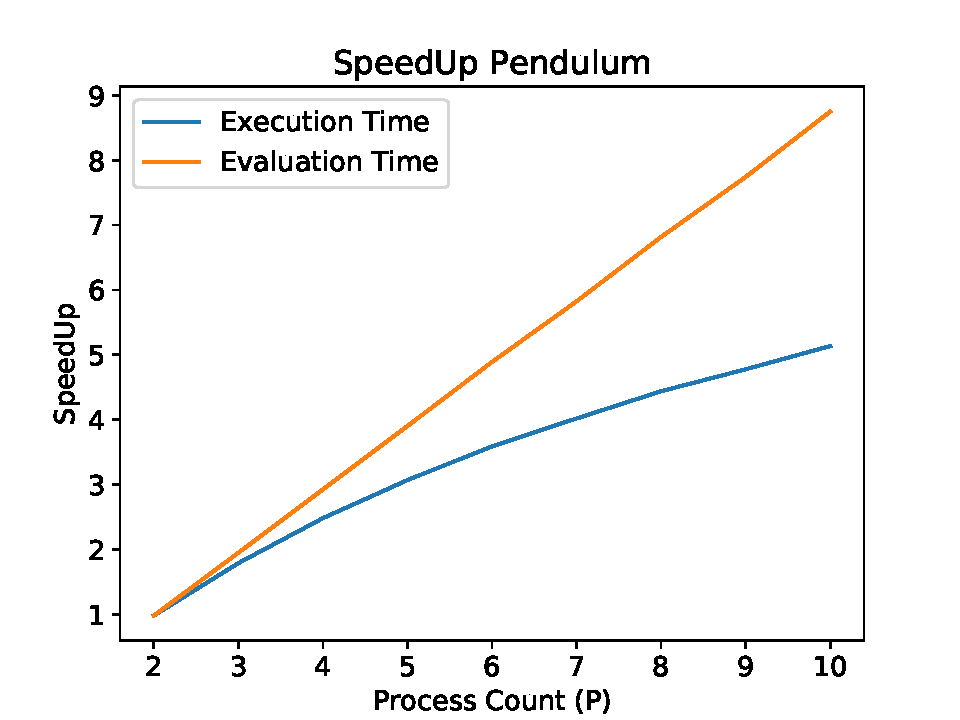
\includegraphics[width=1.0\textwidth]{./img/pendulum_analysis/pendulum_speedup1_2_10.pdf} 
	\end{minipage}
	\hfill
	\begin{minipage}[]{0.49\textwidth}
		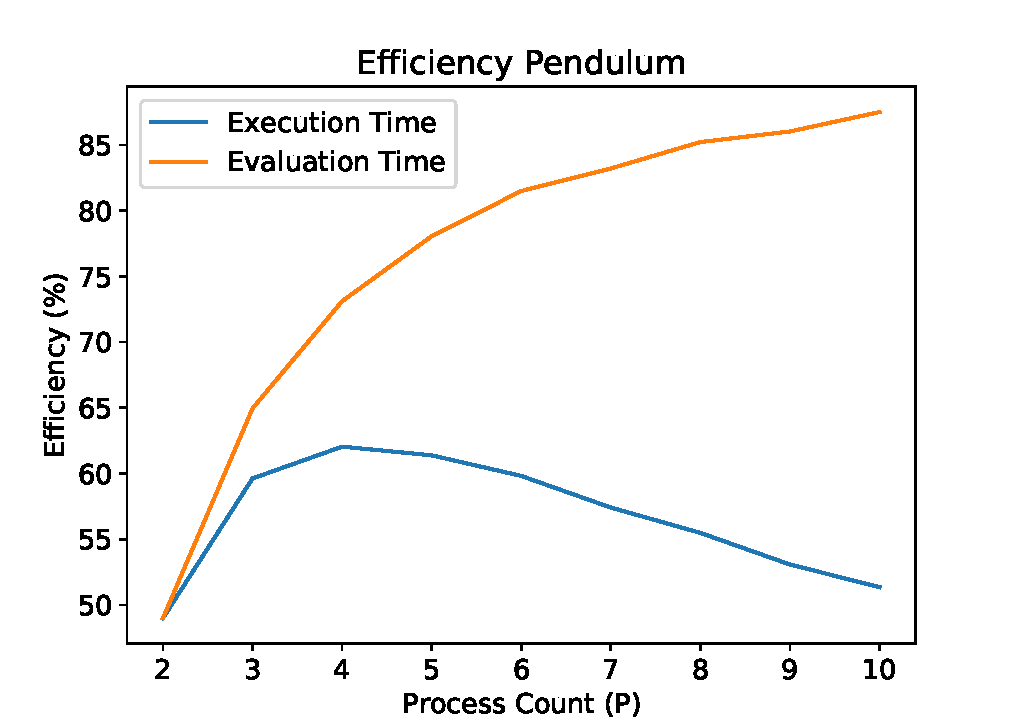
\includegraphics[width=1.0\textwidth]{./img/pendulum_analysis/efficiency_pendulum_2_10.pdf} 
	\end{minipage}
	\caption{Links der \emph{SpeedUp}, rechts die dazugehörigen Effizienzwerte für die \emph{Pendulum} Umgebung in Abhängigkeit der Prozessanzahl}
	\label{fig:pendulum_2_10_efficiency_speedup}
\end{figure}
\\\\
Um die Ausführungszeiten und den Grad der Parallelisierung besser bewerten zu können, wird der \emph{SpeedUp} und die Effizienz für jeden Durchlauf berechnet. Die Ergebnisse sind in Abbildung \ref{fig:pendulum_2_10_efficiency_speedup} dargestellt, wobei jeweils die Werte für das gesamte Verfahren und die parallelisierte \emph{Evaluation Time} dargestellt sind. Auf letzteres wird zuerst eingegangen. Der \emph{SpeedUp} für die Evaluationsphase ist nahezu konstant. Mit zehn Prozessen wird ein Faktor von $8.75$ erzielt. Dieses Ergebnis ähnelt dem der \emph{Mountain Car} Umgebung, in welcher für dieselbe Phase ein Faktor von $8.7$ erreicht wird. Das Ergebnis ist insgesamt sehr gut, da in der \emph{Master-Slave} mit zehn Prozessen bzw. neun \emph{Slaves} der maximal erreichbare \emph{SpeedUp} $9$ beträgt. Dies spiegelt sich auch in der Effizienz wieder. Durch die \emph{Master-Slave} Architektur ist diese initial bei $49\%$, steigt aber steig an. Mit zehn Prozessen wird ein Wert von $87\%$ für die Parallelisierung der \emph{Evaluation Time} erzielt. Die vergleichsweise schlechten initialen Messwerte sind durch den \emph{Master} zu erklären, der zwar in der Berechnung berücksichtigt wird, aber keine Agenten evaluiert. Dasselbe Verhalten tritt in der \emph{Mountain Car} Umgebung auf. Werden bei der Berechnung nur die zur Verfügung stehenden \emph{Slaves} betrachtet, liegt die Effizienz in allen Testdurchläufen bei ungefähr $97\%$, mit einem Maximum von $98\%$. Die fehlenden Prozentpunkte entstehen durch die notwendige Kommunikation. Zusammenfassend zeigen diese Ergebnisse, dass die Parallelisierung der \emph{Evaluation Time} in beiden Testdurchläufen sehr gute und konstante Ergebnisse liefert. Es ist davon auszugehen, dass trotz Hinzufügen von weiteren Prozessen die Effizienz mit einer entsprechenden Populationsgröße weiterhin hoch ist. Hierauf wird im Rahmen des Ergebnisses in Kapitel \ref{sec:results_optimziation} genauer eingegangen. Allerdings ist in der Abbildung \ref{fig:pendulum_2_10_efficiency_speedup} nicht die der \emph{SpeedUp} und die Effizienz für die Evaluationsphase zu sehen, sondern auch für das gesamte Verfahren. Die hierbei erhaltenen Werte sind nicht so gut wie in der \emph{Mountain Car} Umgebung. Mit zehn Prozessen wird ein \emph{SpeedUp} von $5.1$ erreicht. Die \emph{Mountain Car} Umgebung hat im Vergleich hierzu noch einen Wert von $7.6$ erzielt. Auch die Steigung des \emph{SpeedUps} sinkt innerhalb der ersten zehn Generationen drastisch. Grund hierfür ist der Anteil der nicht parallelisierten \emph{Reproduction Time} und \emph{Compose Offspring Time}. Wie in Kapitel \ref{sec:parallel_strategies} veranschaulicht, ist in der \emph{Pendulum} Umgebung ein maximaler \emph{SpeedUp} von $11.\overline{1}$ möglich. Mit steigender Anzahl an Prozessen wird sich das Ergebnis diesem Wert weiter annähern. 
\\\\
Entsprechend des \emph{SpeedUps} sind auch die Effizienzwerte nicht so gut wie in der \emph{Mountain Car} Umgebung. Anfänglich ist diese bei $42\%$ und steigt an, erreicht mit vier Prozessen das Maximum von $62\%$ und sinkt danach kontinuierlich. Hierfür sind dieseleben Gründe verantwortlich wie bei der \emph{Mountain Car} Umgebung. Um die erhaltenen Ergebnisse besser einordnen zu können, werden mit \emph{Amdahl's Law} die erwarteten Effizienzwerte berechnet. Diese sind in Abbildung \ref{fig:pendulumr_efficiency_predidction} dargestellt. Aufgrund der unterschiedlichen Wertebereiche an den Achsen, ist nicht offensichtlich, dass die gemessenen und idealen Ergebnisse sehr ähneln. Die maximal erreichbare Effizienz von ungefähr $63.5\%$ tritt ebenfalls mit vier Prozessen auf. Die restlichen Effizienzwerte für zwei bis zehn Prozesse weichen weniger als zwei Prozentpunkte von dem tatsächlich erhaltenen Ergebnis ab. 
\begin{figure}[!h]
	\centering
	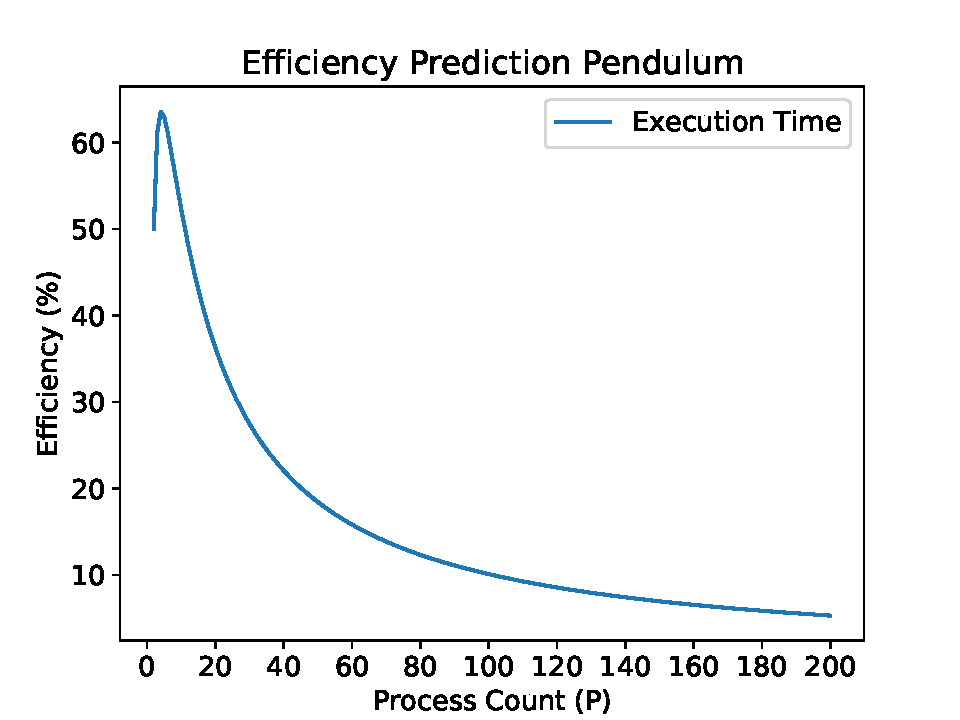
\includegraphics[width=0.7\textwidth]{./img/pendulum_analysis/pendulum_efficiency_prediction.pdf} 
	\caption{Erwartete Effizienz in der \emph{Pendulum} Umgebung in Abhängigkeit der Anzahl an Prozessen}
	\label{fig:pendulumr_efficiency_predidction}
\end{figure}


% Prozentsatz an Abweidung nicht parllelisierter Verfahren, 
% Zuerst Ergebnisse 10 Pis, mit Verifizierung Funktionalität und allgemeines Ergebnis
% Eingehen dass Master Pi keine Abarbeitugn übernimmt sondern nur Koordination
% Zeiten von anderen Phasen weichen ab, daher kann es zu varianzen kommen
% Allgemeine Laufzeit des Verfahrens und Laufzeit des evaluierten Verfahren anzeigen
% Vergleich mit Amdahls Law? +++++ 
